\chapter{Random Sampling}
\label{kap3}

Dieses Kapitel geht auf die konzeptionellen Aspekte des Random Samplings ein. Zunächst betrachtet die Arbeit, weshalb der Algorithmus die beste Wahl für den Laufplaner ist. Darauf folgt die Darstellung der Funktionsweise des Random Samplings, welches große Mengen an zufälligen und gültigen Lösungen generiert.  Dabei sind zwei Fragen von großer Bedeutung. Zum einen ist das: Wie können zufällige gültige Lösungen generiert werden. Wenn diese Lösungen vorliegen ist die nächste wichtige Frage: Wie können diese Lösungen bewertet werden?

Das Kapitel basiert auf der Arbeit von André Herms \autocite{herms2004}, der verschiedene planende Verfahren vorstellt und mit geeigneten Kriterien bewertet. Da seine Arbeit zusammenfassend davon ausgeht, dass Random Sampling die nach seinen Kriterien beste Wahl darstellt, nutzt auch diese Arbeit den Algorithmus.

\section{Kriterien zur Auswahl des Algorithmus}

Herms stellt in seiner Arbeit neben dem Random Sampling die folgenden Algorithmen vor:
\begin{itemize}
  \item \emph{Greedy Verfahren:} Es werden nacheinander Teillösungen durch ein lokales Kriterium generiert. Teillösungen werden nicht mehr verworfen. Daher kommt auch der Begriff "`greedy"', da der Algorithmus gierig ist und somit Lösungen nicht wieder verwirft.
  \item \emph{Branch and Bound:} Das Verfahren liefert durch einen modifzierten Backtracking-Ansatz immer die exakte Lösung. Anders als beim Backtracking werden die Suchbäume gestutzt, so dass die Laufzeit dadurch verkürzt wird.
  \item \emph{Lokale Suche:} Das Verfahren ist eine modifzierte Variante des Random Samplings. Neben der zufälligen Generierung von Lösungen wird auch iterativ in der Nachbarschaft nach einem besseren Punkt geschaut.
  \item \emph{Tabu-Suche:} Das Verfahren ist eine Erweiterung der lokalen Suche. Der Nachbar muss nicht zwingend besser bewertet sein, um als Nachfolgepunkt akzeptiert zu werden. Damit bleibt der Algorithmus nicht in lokalen Maxima hängen.
  \item \emph{Simulated Annealing:} Das Verfahren ist eine erneute Verbesserung der lokalen Suche und der Tabu-Suche, das sich hinsichtlich des Optimierungsproblems an dem physikalischen Prozess des langsamen Abkühlen fester Stoffe orientiert.
  \item \emph{Genetische Algorithmen:} Das Verfahren nutzt die Mechanismen der natürlichen Evolution und wendet diese auf das Problem der Laufplanung an.
\end{itemize}

Die genannten Algorithmen vergleicht Herms nun unter Berücksichtigung der folgenden Kriterien:
\begin{itemize}
  \item Parallelisierbarkeit
  \item Speicherbedarf
  \item Anytime-Fähigkeit
  \item Allgemeine Anwendbarkeit
\end{itemize}

\begin{table}[!t]
  \caption{Bewertung des Random Samplings}
  \label{Kap3:BewertungRandomSampling}
  \renewcommand{\arraystretch}{1.2}
  \centering
  \sffamily
  \begin{footnotesize}
    \begin{tabularx}{0.9\textwidth}{l X}
      \toprule
      \textbf{Kriterium} & \textbf{Erfüllung}\\
      \midrule
      \emph{Parallelisierbarkeit} & Lösungen können ohne großen Aufwand unabhängig voneinander generiert werden. Am Ende müssen diese nur noch synchronisiert werden, so dass die Lösung mit der besten Bewertung übernommen wird.\\
      \emph{Speicherbedarf} & Der Algorithmus benötigt kaum Speicher, da immer nur eine Lösung generiert wird und diese die vorherige beste Lösung überschreibt.\\
      \emph{Anytime} & Das Kriterium ist erfüllt, sobald eine Lösung generiert ist. Allerdings kann es passieren, dass in einer bestimmten Zeit noch keine gute Lösung vorhanden ist.\\
      \emph{Anwendbarkeit} & Der Algorithmus lässt sich auf jedes Problem der Laufplanung anwenden. Die Qualität hängt allerdings vom Anteil guter Lösungen, die im Lösungsraum vorhanden sind. Außerdem spielt die konkrete Implementierung des Algorithmus eine große Rolle. Insgesamt gilt, dass je länger der Algorithmus läuft, desto besser sind potentiell die Lösungen.\\
      \bottomrule
    \end{tabularx}
  \end{footnotesize}
  \rmfamily
\end{table}

Dabei stellt sich heraus, dass nur die Algorithmen \emph{Random Sampling}, \emph{Lokale Suche} und \emph{Simulated Annealing} alle Kriterien mindestens erfüllen. Nach der Implementierung und erster Tests stellt sich heraus, dass das Random Sampling die Kriterien am besten erfüllt, da die Lokale Suche sowie das Simulated Annealing die Lösungen zu langsam erstellen. \autoref{Kap3:BewertungRandomSampling} zeigt die weiteren Kriterien, die für die Bewertung des Algorithmus wichtig sind. Auch hier schneidet das Random Sampling positiv ab.

Zusammenfassend ist nun festzuhalten, dass das Random Sampling für den Laufplaner genutzt werden soll, da es zwischen allen Algorithmen am besten abschneidet.

\section{Erzeugen gültiger Lösungen}

Der Algorithmus zur Erzeugung gültiger Lösungen für die Gesamtstrecke wurde initial von André Herms \autocite{herms2004} entwickelt. Uli Ruffler \autocite{ruffler2006} hat diesen in seiner Arbeit unter anderem dahingehend weiterentwickelt, dass dieser auf einer inkrementellen Arbeitsweise läuft. Der folgende Abschnitt geht nun auf das grundlegende Konzept der Generierung von gültigen Lösungen ein.

Wichtig ist, dass alle möglichen Lösungen generiert werden können und nur Lösungen ausgeschlossen werden, die außerhalb des gültigen Bereichs der Fußwinkel und Fußgeschwindigkeiten liegen, die auf instabilem Untergrund wie einem zu starkem Gefälle liegen und die den Roboter zum Umkippen bringen würden.

Das Generieren von Lösungen erfolgt nun in mehreren Schritten. Zu Beginn müssen einige Berechnungen für die Festlegung des Pfades zum Ziel ablaufen, bevor der Hauptteil des Algorithmus abläuft, welcher sich schrittweise an das Ziel nähert, bis der Abstand zum Ziel annähernd null beträgt.

\subsection{Festlegung des Pfades zum Ziel}

Eine erste Methode ist es, den Weg vom Start zum Ziel auf direktem Weg zu erreichen. Da allerdings nicht immer Lösungen auf direktem Weg möglich sind, müssen auch andere Pfade generiert werden. Beispielsweise könnte ein unüberwindbarer Graben oder eine hohe Mauer dafür sorgen, dass kein direkter Weg möglich ist. In diesem Fall müsste der Laufroboter den Weg um das Hindernis planen, um eine gültige Lösung zu finden. Um nun alle Fälle abzudecken, benötigt man eine zufällige Streckenplanung. Diese erfolgt, indem zuerst die Anzahl der Pfadsegmente festgelegt wird und dann genau so viele Wegpunkte gesetzt werden.

\subsubsection{Festlegung der Anzahl der Pfadsegmente}

Die Festlegung der Anzahl der Pfadsegmente erfolgt über eine \emph{geometrische Verteilung}. Diese Verteilung wird genutzt, da geringe Streckenanzahlen häufig sein sollen, da davon ausgangen wird, dass der direkte Weg der schnellste Weg ist. Höhere Streckenanzahlen sollen weniger oft auftreten. Durch die Veränderung des Parameters $p$ lassen sich die Wahrscheinlichkeiten dahingehend variieren, dass entweder höhere oder niedrigere Streckenanzahlen bevorzugt werden. Standardmäßig geht man von $p = 0.5$ aus, was bedeutet, dass die Wahrscheinlichkeit genau einen Streckenabschnitt zu erhalten 50\% beträgt.

\subsubsection{Festlegung der Wegpunkte}

Nun ist definiert, wie viele Segmente der Pfad haben soll. Jetzt müssen die Wegpunkte auf dem Pfad zufällig generiert werden. Für jeden Pfadpunkt $P$ wird einzeln eine Lösung generiert. Zunächst wird der Mittelpunkt $m(x, y)$ sowie die Länge $l$ zwischen Start und Ende berechnet. Auf den Mittelpunkt wird nun ein zufälliger Vektor $r(x, y)$ addiert, dessen generierter Wert vom negativen bis zum positiven Betrag der Länge $l$ reicht. \autoref{RandomSamplingWegpunkteP1} und \autoref{RandomSamplingWegpunkteP2} zeigen mögliche Ergebnisse für drei Pfadsegmente $P_1$, $P_2$ und $P_3$ für den Startpunkt $S(0,0)$ und dem Zielpunkt $Z(10,0)$. Der letzte Pfadpunkt $P_3$ entspricht immer genau der Zielposition, damit der Roboter dieses Ziel in jedem Fall erreicht. \autoref{Kap3:RSWegpunkte} zeigt die generierten Punkte und damit den Pfad des Roboters grafisch dargestellt.

\begin{equation}
  P_1=\left(\begin{array}{c} x_m + x_r \\ y_m + y_r \end{array}\right)=\left(\begin{array}{c} 5 - 2.31 \\ 0 - 4.1 \end{array}\right)=\left(\begin{array}{c} 3.31 \\ -4.1 \end{array}\right) \qquad
\label{RandomSamplingWegpunkteP1}
\end{equation}

\begin{equation}
  P_2=\left(\begin{array}{c} x_m + x_r \\ y_m + y_r \end{array}\right)=\left(\begin{array}{c} 5 + 3.1 \\ 0 + 0.5 \end{array}\right)=\left(\begin{array}{c} 8.1 \\ 0.5 \end{array}\right) \qquad
\label{RandomSamplingWegpunkteP2}
\end{equation}

\begin{figure}[t]
  \centering
  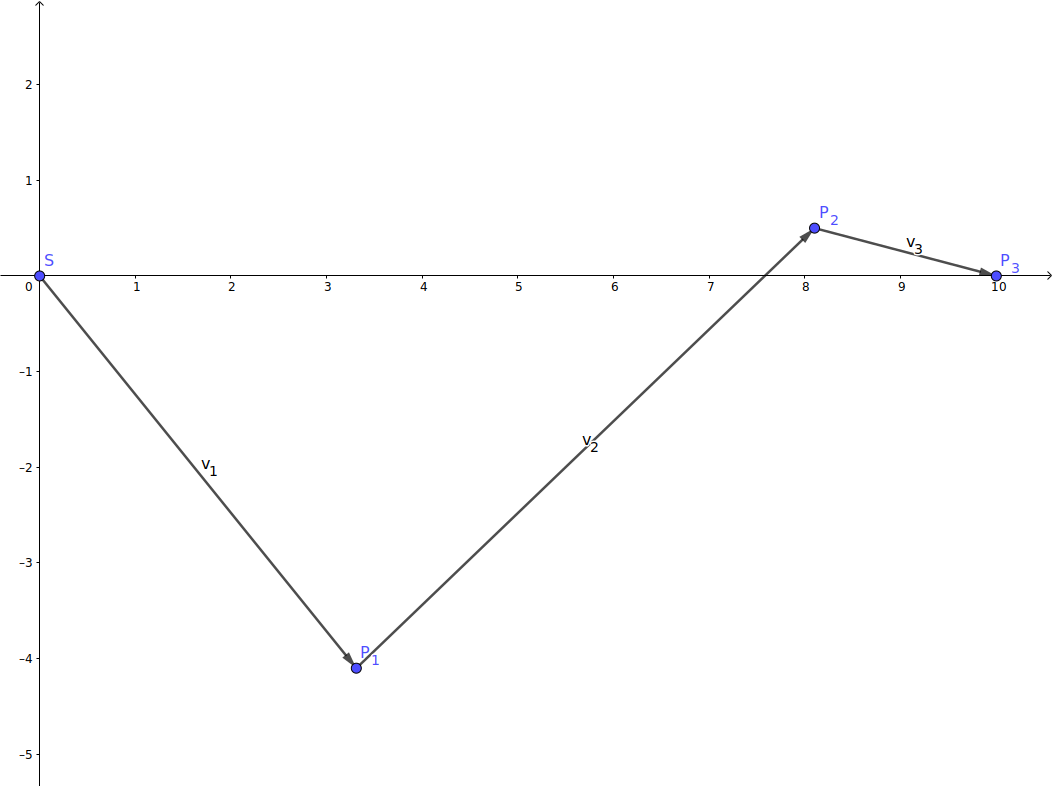
\includegraphics[height=10cm]{kapitel3/rswegpunkte}
  \caption{Zufällig generierte Wegpunkte}
  \label{Kap3:RSWegpunkte}
\end{figure}

Mit dieser Berechnung sind nun für den Mittelpunkt des Körpers des Laufroboters ausschließlich Bewegungen auf diesem Pfad möglich. Bewusst wird hier noch nicht mit der z-Koordinate gearbeitet, da diese je nach Fußstellung und Terrain variiert.

\subsection{Schrittweise Näherung an das Ziel}

Die schrittweise Näherung an das Ziel erfolgt solange, bis der Abstand zum Ziel minimal ist. Ein exakter Vergleich mit dem Abstand null ist nicht effektiv, da der Roboter sonst fortwährend versuchen würde auf seine Zielposition zu gelangen, aber ununterbrochen minimale Abweichungen zum Ziel hätte, was den Prozess erneut anstoßen würde. Der Ablauf, um die Füße anzuheben oder abzusetzen sowie den Körper zu bewegen, läuft folgendermaßen ab:
\begin{enumerate}
  \item Berechnung des zulässigen Bereichs
  \item Auswahl der nächsten Fuß-Konfiguration
\end{enumerate}

Neben den zwei Schritten nennt André Herms \autocite{herms2004} noch zwei weitere Schritt zur Berechnung der Mittelpunktpositionen und der Festlegung der Dauer der Bewegungen. Dieser werden erst nach der schrittweisen Näherung an das Ziel durchgeführt.

\subsubsection{Berechnung des zulässigen Bereichs}

Der zulässige Bereich des Mittelpunkts ist auf Grund von zwei Kriterien eingeschränkt. Zum einen durch der maximalen Reichweite der Fußpunkte vom Mittelpunkt aus. Zum anderen dadurch, dass der minimale \emph{Stability Margin} nicht unterschritten werden darf. Der Stability Margin ist der kleinste Abstand zum Mittelpunkt der konvexen Hülle der Fußpunkte vom Mittelpunkt aus. Dieser ist ein Maß dafür, wie stabil der Roboter steht. Ist der Stability Margin kleiner als null, so ist der Mittelpunkt außerhalb der konvexen Hülle, was ein Kippen des Roboters verursacht. Je größer der Stability Margin, desto stabiler steht der Roboter.

Der zulässige Bereich kann nur an zwei Punkten verlassen werden. Damit wird ein Start- und ein Endpunkt der aktuellen Fußstellung gebildet. Diese sind analytisch schwer zu berechnen. Daher muss mit einem numerischen Verfahren, der \emph{binären Suche}, mit einem inneren zulässigen Punkt und einem äußerem unzulässigen Punkt der Schnittpunkt mit dem zulässigen Bereich gesucht werden. Dazu genügt eine Funktion welche angibt, ob der Mittelpunkt zulässig oder unzulässig ist.

\subsubsection{Auswahl der nächsten Fuß-Konfiguration}

Der Mittelpunkt des Roboterkörpers kann sich in diesem aktuellen Zustand nur noch vom zuletzt berechneten Start- und Endpunkt des zulässigen Bereichs bewegen. Dies geschieht durch das Verschieben der Körpermitte. Dazu müssen die Füße gehoben und umgesetzt werden. Auch hier müssen die zu Beginn genannten Kriterien beachtet werden. Diese sind unter anderem, dass sich mindestens drei Füße auf dem Boden befinden und dass mindestens ein Fuß auf jeder Seite den Körper stützt, damit der Stability Margin positiv ist. Mit diesen Regeln lassen sich 40 mögliche Fußkonfigurationen, auch Stützzustände genannt, darstellen, welche in \autoref{validconf} abgebildet sind.

\begin{table}[ht!]
\setlength{\unitlength}{.9cm}
\begin{picture}(1.5,3.5)
\put(0.25,0.25){\dashbox{0.05}(1,2){} }
\put(0.25,1.25){\circle*{0.2}}
\put(1.25,1.25){\circle*{0.2}}
\put(1.25,0.25){\circle*{0.2}}
\put(1.25,0.25){\line(0,1){1}}
\put(0.25,1.25){\line(0,0){0}}
\put(0.25,1.25){\line(1, -1){1}}
\put(0.25,1.25){\line(1, 0){1}}
\put(0.75,2.5){\makebox(0,0)[b]{1}}
\end{picture}
\begin{picture}(1.5,3.5)
\put(0.25,0.25){\dashbox{0.05}(1,2){} }
\put(0.25,1.25){\circle*{0.2}}
\put(1.25,1.25){\circle*{0.2}}
\put(0.25,0.25){\circle*{0.2}}
\put(1.25,1.25){\line(0,0){0}}
\put(0.25,0.25){\line(0,1){1}}
\put(0.25,0.25){\line(1, 1){1}}
\put(0.25,1.25){\line(1, 0){1}}
\put(0.75,2.5){\makebox(0,0)[b]{2}}
\end{picture}
\begin{picture}(1.5,3.5)
\put(0.25,0.25){\dashbox{0.05}(1,2){} }
\put(0.25,2.25){\circle*{0.2}}
\put(0.25,1.25){\circle*{0.2}}
\put(1.25,1.25){\circle*{0.2}}
\put(1.25,1.25){\line(0,0){0}}
\put(0.25,1.25){\line(0,1){1}}
\put(0.25,1.25){\line(1, 0){1}}
\put(0.25,2.25){\line(1, -1){1}}
\put(0.75,2.5){\makebox(0,0)[b]{3}}
\end{picture}
\begin{picture}(1.5,3.5)
\put(0.25,0.25){\dashbox{0.05}(1,2){} }
\put(1.25,2.25){\circle*{0.2}}
\put(0.25,1.25){\circle*{0.2}}
\put(1.25,1.25){\circle*{0.2}}
\put(1.25,1.25){\line(0,1){1}}
\put(0.25,1.25){\line(0,0){0}}
\put(0.25,1.25){\line(1, 0){1}}
\put(0.25,1.25){\line(1, 1){1}}
\put(0.75,2.5){\makebox(0,0)[b]{4}}
\end{picture}
\begin{picture}(1.5,3.5)
\put(0.25,0.25){\dashbox{0.05}(1,2){} }
\put(1.25,1.25){\circle*{0.2}}
\put(0.25,0.25){\circle*{0.2}}
\put(1.25,0.25){\circle*{0.2}}
\put(1.25,0.25){\line(0,1){1}}
\put(0.25,0.25){\line(0,0){0}}
\put(0.25,0.25){\line(1, 0){1}}
\put(0.25,0.25){\line(1, 1){1}}
\put(0.75,2.5){\makebox(0,0)[b]{5}}
\end{picture}
\begin{picture}(1.5,3.5)
\put(0.25,0.25){\dashbox{0.05}(1,2){} }
\put(0.25,1.25){\circle*{0.2}}
\put(0.25,0.25){\circle*{0.2}}
\put(1.25,0.25){\circle*{0.2}}
\put(1.25,0.25){\line(0,0){0}}
\put(0.25,0.25){\line(0,1){1}}
\put(0.25,0.25){\line(1, 0){1}}
\put(0.25,1.25){\line(1, -1){1}}
\put(0.75,2.5){\makebox(0,0)[b]{6}}
\end{picture}
\begin{picture}(1.5,3.5)
\put(0.25,0.25){\dashbox{0.05}(1,2){} }
\put(0.25,2.25){\circle*{0.2}}
\put(1.25,2.25){\circle*{0.2}}
\put(1.25,1.25){\circle*{0.2}}
\put(1.25,1.25){\line(0,1){1}}
\put(0.25,2.25){\line(0,0){0}}
\put(0.25,2.25){\line(1, -1){1}}
\put(0.25,2.25){\line(1, 0){1}}
\put(0.75,2.5){\makebox(0,0)[b]{7}}
\end{picture}
\begin{picture}(1.5,3.5)
\put(0.25,0.25){\dashbox{0.05}(1,2){} }
\put(0.25,2.25){\circle*{0.2}}
\put(1.25,2.25){\circle*{0.2}}
\put(0.25,1.25){\circle*{0.2}}
\put(1.25,2.25){\line(0,0){0}}
\put(0.25,1.25){\line(0,1){1}}
\put(0.25,1.25){\line(1, 1){1}}
\put(0.25,2.25){\line(1, 0){1}}
\put(0.75,2.5){\makebox(0,0)[b]{8}}
\end{picture}
\begin{picture}(1.5,3.5)
\put(0.25,0.25){\dashbox{0.05}(1,2){} }
\put(1.25,2.25){\circle*{0.2}}
\put(1.25,1.25){\circle*{0.2}}
\put(0.25,0.25){\circle*{0.2}}
\put(1.25,1.25){\line(0,1){1}}
\put(0.25,0.25){\line(0,0){0}}
\put(0.25,0.25){\line(1, 1){1}}
\put(0.25,0.25){\line(1, 2){1}}
\put(0.75,2.5){\makebox(0,0)[b]{9}}
\end{picture}
\begin{picture}(1.5,3.5)
\put(0.25,0.25){\dashbox{0.05}(1,2){} }
\put(1.25,2.25){\circle*{0.2}}
\put(0.25,1.25){\circle*{0.2}}
\put(0.25,0.25){\circle*{0.2}}
\put(1.25,2.25){\line(0,0){0}}
\put(0.25,0.25){\line(0,1){1}}
\put(0.25,0.25){\line(1, 2){1}}
\put(0.25,1.25){\line(1, 1){1}}
\put(0.75,2.5){\makebox(0,0)[b]{10}}
\end{picture}
\begin{picture}(1.5,3.5)
\put(0.25,0.25){\dashbox{0.05}(1,2){} }
\put(0.25,2.25){\circle*{0.2}}
\put(1.25,1.25){\circle*{0.2}}
\put(1.25,0.25){\circle*{0.2}}
\put(1.25,0.25){\line(0,1){1}}
\put(0.25,2.25){\line(0,0){0}}
\put(0.25,2.25){\line(1, -2){1}}
\put(0.25,2.25){\line(1, -1){1}}
\put(0.75,2.5){\makebox(0,0)[b]{11}}
\end{picture}
\begin{picture}(1.5,3.5)
\put(0.25,0.25){\dashbox{0.05}(1,2){} }
\put(0.25,2.25){\circle*{0.2}}
\put(0.25,1.25){\circle*{0.2}}
\put(1.25,0.25){\circle*{0.2}}
\put(1.25,0.25){\line(0,0){0}}
\put(0.25,1.25){\line(0,1){1}}
\put(0.25,1.25){\line(1, -1){1}}
\put(0.25,2.25){\line(1, -2){1}}
\put(0.75,2.5){\makebox(0,0)[b]{12}}
\end{picture}
\begin{picture}(1.5,3.5)
\put(0.25,0.25){\dashbox{0.05}(1,2){} }
\put(0.25,2.25){\circle*{0.2}}
\put(1.25,2.25){\circle*{0.2}}
\put(1.25,0.25){\circle*{0.2}}
\put(1.25,0.25){\line(0,2){2}}
\put(0.25,2.25){\line(0,0){0}}
\put(0.25,2.25){\line(1, -2){1}}
\put(0.25,2.25){\line(1, 0){1}}
\put(0.75,2.5){\makebox(0,0)[b]{13}}
\end{picture}
\begin{picture}(1.5,3.5)
\put(0.25,0.25){\dashbox{0.05}(1,2){} }
\put(1.25,2.25){\circle*{0.2}}
\put(0.25,0.25){\circle*{0.2}}
\put(1.25,0.25){\circle*{0.2}}
\put(1.25,0.25){\line(0,2){2}}
\put(0.25,0.25){\line(0,0){0}}
\put(0.25,0.25){\line(1, 0){1}}
\put(0.25,0.25){\line(1, 2){1}}
\put(0.75,2.5){\makebox(0,0)[b]{14}}
\end{picture}
\begin{picture}(1.5,3.5)
\put(0.25,0.25){\dashbox{0.05}(1,2){} }
\put(0.25,2.25){\circle*{0.2}}
\put(1.25,2.25){\circle*{0.2}}
\put(0.25,0.25){\circle*{0.2}}
\put(1.25,2.25){\line(0,0){0}}
\put(0.25,0.25){\line(0,2){2}}
\put(0.25,0.25){\line(1, 2){1}}
\put(0.25,2.25){\line(1, 0){1}}
\put(0.75,2.5){\makebox(0,0)[b]{15}}
\end{picture}
\begin{picture}(1.5,3.5)
\put(0.25,0.25){\dashbox{0.05}(1,2){} }
\put(0.25,2.25){\circle*{0.2}}
\put(0.25,0.25){\circle*{0.2}}
\put(1.25,0.25){\circle*{0.2}}
\put(1.25,0.25){\line(0,0){0}}
\put(0.25,0.25){\line(0,2){2}}
\put(0.25,0.25){\line(1, 0){1}}
\put(0.25,2.25){\line(1, -2){1}}
\put(0.75,2.5){\makebox(0,0)[b]{16}}
\end{picture}
\begin{picture}(1.5,3.5)
\put(0.25,0.25){\dashbox{0.05}(1,2){} }
\put(1.25,2.25){\circle*{0.2}}
\put(0.25,1.25){\circle*{0.2}}
\put(1.25,0.25){\circle*{0.2}}
\put(1.25,0.25){\line(0,2){2}}
\put(0.25,1.25){\line(0,0){0}}
\put(0.25,1.25){\line(1, -1){1}}
\put(0.25,1.25){\line(1, 1){1}}
\put(0.75,2.5){\makebox(0,0)[b]{17}}
\end{picture}
\begin{picture}(1.5,3.5)
\put(0.25,0.25){\dashbox{0.05}(1,2){} }
\put(0.25,2.25){\circle*{0.2}}
\put(1.25,1.25){\circle*{0.2}}
\put(0.25,0.25){\circle*{0.2}}
\put(1.25,1.25){\line(0,0){0}}
\put(0.25,0.25){\line(0,2){2}}
\put(0.25,0.25){\line(1, 1){1}}
\put(0.25,2.25){\line(1, -1){1}}
\put(0.75,2.5){\makebox(0,0)[b]{18}}
\end{picture}
\begin{picture}(1.5,3.5)
\put(0.25,0.25){\dashbox{0.05}(1,2){} }
\put(0.25,2.25){\circle*{0.2}}
\put(0.25,1.25){\circle*{0.2}}
\put(1.25,1.25){\circle*{0.2}}
\put(0.25,0.25){\circle*{0.2}}
\put(1.25,1.25){\line(0,0){0}}
\put(0.25,0.25){\line(0,2){2}}
\put(0.25,0.25){\line(1, 1){1}}
\put(0.25,2.25){\line(1, -1){1}}
\put(0.75,2.5){\makebox(0,0)[b]{19}}
\end{picture}
\begin{picture}(1.5,3.5)
\put(0.25,0.25){\dashbox{0.05}(1,2){} }
\put(1.25,2.25){\circle*{0.2}}
\put(0.25,1.25){\circle*{0.2}}
\put(1.25,1.25){\circle*{0.2}}
\put(1.25,0.25){\circle*{0.2}}
\put(1.25,0.25){\line(0,2){2}}
\put(0.25,1.25){\line(0,0){0}}
\put(0.25,1.25){\line(1, -1){1}}
\put(0.25,1.25){\line(1, 1){1}}
\put(0.75,2.5){\makebox(0,0)[b]{20}}
\end{picture}
\begin{picture}(1.5,3.5)
\put(0.25,0.25){\dashbox{0.05}(1,2){} }
\put(1.25,2.25){\circle*{0.2}}
\put(1.25,1.25){\circle*{0.2}}
\put(0.25,0.25){\circle*{0.2}}
\put(1.25,0.25){\circle*{0.2}}
\put(1.25,0.25){\line(0,2){2}}
\put(0.25,0.25){\line(0,0){0}}
\put(0.25,0.25){\line(1, 0){1}}
\put(0.25,0.25){\line(1, 2){1}}
\put(0.75,2.5){\makebox(0,0)[b]{21}}
\end{picture}
\begin{picture}(1.5,3.5)
\put(0.25,0.25){\dashbox{0.05}(1,2){} }
\put(0.25,2.25){\circle*{0.2}}
\put(0.25,1.25){\circle*{0.2}}
\put(0.25,0.25){\circle*{0.2}}
\put(1.25,0.25){\circle*{0.2}}
\put(1.25,0.25){\line(0,0){0}}
\put(0.25,0.25){\line(0,2){2}}
\put(0.25,0.25){\line(1, 0){1}}
\put(0.25,2.25){\line(1, -2){1}}
\put(0.75,2.5){\makebox(0,0)[b]{22}}
\end{picture}
\begin{picture}(1.5,3.5)
\put(0.25,0.25){\dashbox{0.05}(1,2){} }
\put(0.25,2.25){\circle*{0.2}}
\put(1.25,2.25){\circle*{0.2}}
\put(1.25,1.25){\circle*{0.2}}
\put(1.25,0.25){\circle*{0.2}}
\put(1.25,0.25){\line(0,2){2}}
\put(0.25,2.25){\line(0,0){0}}
\put(0.25,2.25){\line(1, -2){1}}
\put(0.25,2.25){\line(1, 0){1}}
\put(0.75,2.5){\makebox(0,0)[b]{23}}
\end{picture}
\begin{picture}(1.5,3.5)
\put(0.25,0.25){\dashbox{0.05}(1,2){} }
\put(0.25,2.25){\circle*{0.2}}
\put(1.25,2.25){\circle*{0.2}}
\put(0.25,1.25){\circle*{0.2}}
\put(0.25,0.25){\circle*{0.2}}
\put(1.25,2.25){\line(0,0){0}}
\put(0.25,0.25){\line(0,2){2}}
\put(0.25,0.25){\line(1, 2){1}}
\put(0.25,2.25){\line(1, 0){1}}
\put(0.75,2.5){\makebox(0,0)[b]{24}}
\end{picture}
\begin{picture}(1.5,3.5)
\put(0.25,0.25){\dashbox{0.05}(1,2){} }
\put(0.25,2.25){\circle*{0.2}}
\put(1.25,2.25){\circle*{0.2}}
\put(0.25,1.25){\circle*{0.2}}
\put(1.25,1.25){\circle*{0.2}}
\put(1.25,1.25){\line(0,1){1}}
\put(0.25,1.25){\line(0,1){1}}
\put(0.25,1.25){\line(1, 0){1}}
\put(0.25,2.25){\line(1, 0){1}}
\put(0.75,2.5){\makebox(0,0)[b]{25}}
\end{picture}
\begin{picture}(1.5,3.5)
\put(0.25,0.25){\dashbox{0.05}(1,2){} }
\put(0.25,1.25){\circle*{0.2}}
\put(1.25,1.25){\circle*{0.2}}
\put(0.25,0.25){\circle*{0.2}}
\put(1.25,0.25){\circle*{0.2}}
\put(1.25,0.25){\line(0,1){1}}
\put(0.25,0.25){\line(0,1){1}}
\put(0.25,0.25){\line(1, 0){1}}
\put(0.25,1.25){\line(1, 0){1}}
\put(0.75,2.5){\makebox(0,0)[b]{26}}
\end{picture}
\begin{picture}(1.5,3.5)
\put(0.25,0.25){\dashbox{0.05}(1,2){} }
\put(1.25,2.25){\circle*{0.2}}
\put(0.25,1.25){\circle*{0.2}}
\put(1.25,1.25){\circle*{0.2}}
\put(0.25,0.25){\circle*{0.2}}
\put(1.25,1.25){\line(0,1){1}}
\put(0.25,0.25){\line(0,1){1}}
\put(0.25,0.25){\line(1, 1){1}}
\put(0.25,1.25){\line(1, 1){1}}
\put(0.75,2.5){\makebox(0,0)[b]{27}}
\end{picture}
\begin{picture}(1.5,3.5)
\put(0.25,0.25){\dashbox{0.05}(1,2){} }
\put(0.25,2.25){\circle*{0.2}}
\put(0.25,1.25){\circle*{0.2}}
\put(1.25,1.25){\circle*{0.2}}
\put(1.25,0.25){\circle*{0.2}}
\put(1.25,0.25){\line(0,1){1}}
\put(0.25,1.25){\line(0,1){1}}
\put(0.25,1.25){\line(1, -1){1}}
\put(0.25,2.25){\line(1, -1){1}}
\put(0.75,2.5){\makebox(0,0)[b]{28}}
\end{picture}
\begin{picture}(1.5,3.5)
\put(0.25,0.25){\dashbox{0.05}(1,2){} }
\put(1.25,2.25){\circle*{0.2}}
\put(0.25,1.25){\circle*{0.2}}
\put(0.25,0.25){\circle*{0.2}}
\put(1.25,0.25){\circle*{0.2}}
\put(1.25,0.25){\line(0,2){2}}
\put(0.25,0.25){\line(0,1){1}}
\put(0.25,0.25){\line(1, 0){1}}
\put(0.25,1.25){\line(1, 1){1}}
\put(0.75,2.5){\makebox(0,0)[b]{29}}
\end{picture}
\begin{picture}(1.5,3.5)
\put(0.25,0.25){\dashbox{0.05}(1,2){} }
\put(0.25,2.25){\circle*{0.2}}
\put(1.25,1.25){\circle*{0.2}}
\put(0.25,0.25){\circle*{0.2}}
\put(1.25,0.25){\circle*{0.2}}
\put(1.25,0.25){\line(0,1){1}}
\put(0.25,0.25){\line(0,2){2}}
\put(0.25,0.25){\line(1, 0){1}}
\put(0.25,2.25){\line(1, -1){1}}
\put(0.75,2.5){\makebox(0,0)[b]{30}}
\end{picture}
\begin{picture}(1.5,3.5)
\put(0.25,0.25){\dashbox{0.05}(1,2){} }
\put(0.25,2.25){\circle*{0.2}}
\put(1.25,2.25){\circle*{0.2}}
\put(0.25,1.25){\circle*{0.2}}
\put(1.25,0.25){\circle*{0.2}}
\put(1.25,0.25){\line(0,2){2}}
\put(0.25,1.25){\line(0,1){1}}
\put(0.25,1.25){\line(1, -1){1}}
\put(0.25,2.25){\line(1, 0){1}}
\put(0.75,2.5){\makebox(0,0)[b]{31}}
\end{picture}
\begin{picture}(1.5,3.5)
\put(0.25,0.25){\dashbox{0.05}(1,2){} }
\put(0.25,2.25){\circle*{0.2}}
\put(1.25,2.25){\circle*{0.2}}
\put(1.25,1.25){\circle*{0.2}}
\put(0.25,0.25){\circle*{0.2}}
\put(1.25,1.25){\line(0,1){1}}
\put(0.25,0.25){\line(0,2){2}}
\put(0.25,0.25){\line(1, 1){1}}
\put(0.25,2.25){\line(1, 0){1}}
\put(0.75,2.5){\makebox(0,0)[b]{32}}
\end{picture}
\begin{picture}(1.5,3.5)
\put(0.25,0.25){\dashbox{0.05}(1,2){} }
\put(0.25,2.25){\circle*{0.2}}
\put(1.25,2.25){\circle*{0.2}}
\put(0.25,0.25){\circle*{0.2}}
\put(1.25,0.25){\circle*{0.2}}
\put(1.25,0.25){\line(0,2){2}}
\put(0.25,0.25){\line(0,2){2}}
\put(0.25,0.25){\line(1, 0){1}}
\put(0.25,2.25){\line(1, 0){1}}
\put(0.75,2.5){\makebox(0,0)[b]{33}}
\end{picture}
\begin{picture}(1.5,3.5)
\put(0.25,0.25){\dashbox{0.05}(1,2){} }
\put(1.25,2.25){\circle*{0.2}}
\put(0.25,1.25){\circle*{0.2}}
\put(1.25,1.25){\circle*{0.2}}
\put(0.25,0.25){\circle*{0.2}}
\put(1.25,0.25){\circle*{0.2}}
\put(1.25,0.25){\line(0,2){2}}
\put(0.25,0.25){\line(0,1){1}}
\put(0.25,0.25){\line(1, 0){1}}
\put(0.25,1.25){\line(1, 1){1}}
\put(0.75,2.5){\makebox(0,0)[b]{34}}
\end{picture}
\begin{picture}(1.5,3.5)
\put(0.25,0.25){\dashbox{0.05}(1,2){} }
\put(0.25,2.25){\circle*{0.2}}
\put(0.25,1.25){\circle*{0.2}}
\put(1.25,1.25){\circle*{0.2}}
\put(0.25,0.25){\circle*{0.2}}
\put(1.25,0.25){\circle*{0.2}}
\put(1.25,0.25){\line(0,1){1}}
\put(0.25,0.25){\line(0,2){2}}
\put(0.25,0.25){\line(1, 0){1}}
\put(0.25,2.25){\line(1, -1){1}}
\put(0.75,2.5){\makebox(0,0)[b]{35}}
\end{picture}
\begin{picture}(1.5,3.5)
\put(0.25,0.25){\dashbox{0.05}(1,2){} }
\put(0.25,2.25){\circle*{0.2}}
\put(1.25,2.25){\circle*{0.2}}
\put(0.25,1.25){\circle*{0.2}}
\put(1.25,1.25){\circle*{0.2}}
\put(1.25,0.25){\circle*{0.2}}
\put(1.25,0.25){\line(0,2){2}}
\put(0.25,1.25){\line(0,1){1}}
\put(0.25,1.25){\line(1, -1){1}}
\put(0.25,2.25){\line(1, 0){1}}
\put(0.75,2.5){\makebox(0,0)[b]{36}}
\end{picture}
\begin{picture}(1.5,3.5)
\put(0.25,0.25){\dashbox{0.05}(1,2){} }
\put(0.25,2.25){\circle*{0.2}}
\put(1.25,2.25){\circle*{0.2}}
\put(0.25,1.25){\circle*{0.2}}
\put(1.25,1.25){\circle*{0.2}}
\put(0.25,0.25){\circle*{0.2}}
\put(1.25,1.25){\line(0,1){1}}
\put(0.25,0.25){\line(0,2){2}}
\put(0.25,0.25){\line(1, 1){1}}
\put(0.25,2.25){\line(1, 0){1}}
\put(0.75,2.5){\makebox(0,0)[b]{37}}
\end{picture}
\begin{picture}(1.5,3.5)
\put(0.25,0.25){\dashbox{0.05}(1,2){} }
\put(0.25,2.25){\circle*{0.2}}
\put(1.25,2.25){\circle*{0.2}}
\put(1.25,1.25){\circle*{0.2}}
\put(0.25,0.25){\circle*{0.2}}
\put(1.25,0.25){\circle*{0.2}}
\put(1.25,0.25){\line(0,2){2}}
\put(0.25,0.25){\line(0,2){2}}
\put(0.25,0.25){\line(1, 0){1}}
\put(0.25,2.25){\line(1, 0){1}}
\put(0.75,2.5){\makebox(0,0)[b]{38}}
\end{picture}
\begin{picture}(1.5,3.5)
\put(0.25,0.25){\dashbox{0.05}(1,2){} }
\put(0.25,2.25){\circle*{0.2}}
\put(1.25,2.25){\circle*{0.2}}
\put(0.25,1.25){\circle*{0.2}}
\put(0.25,0.25){\circle*{0.2}}
\put(1.25,0.25){\circle*{0.2}}
\put(1.25,0.25){\line(0,2){2}}
\put(0.25,0.25){\line(0,2){2}}
\put(0.25,0.25){\line(1, 0){1}}
\put(0.25,2.25){\line(1, 0){1}}
\put(0.75,2.5){\makebox(0,0)[b]{39}}
\end{picture}
\begin{picture}(1.5,3.5)
\put(0.25,0.25){\dashbox{0.05}(1,2){} }
\put(0.25,2.25){\circle*{0.2}}
\put(1.25,2.25){\circle*{0.2}}
\put(0.25,1.25){\circle*{0.2}}
\put(1.25,1.25){\circle*{0.2}}
\put(0.25,0.25){\circle*{0.2}}
\put(1.25,0.25){\circle*{0.2}}
\put(1.25,0.25){\line(0,2){2}}
\put(0.25,0.25){\line(0,2){2}}
\put(0.25,0.25){\line(1, 0){1}}
\put(0.25,2.25){\line(1, 0){1}}
\put(0.75,2.5){\makebox(0,0)[b]{40}}
\end{picture}
\caption{\label{validconf}40 zulässige Stützzustände \autocite{herms2004}}
\end{table}

Mit jedem Übergang eines Stützzustands in einen anderen Stützzustands wird exakt ein Fuß entweder angehoben oder abgesetzt. Es können auch mehrere Füße gleichzeitig angehoben oder abgesetzt werden, indem in dem aktuellen Übergang eine Zeitdauer von $t=0s$ angenommen wird. Damit wird der nächste Stützzustand mit dem aktuellen Stützzustand ausgeführt. \autoref{trans_support} gibt alle möglichen Stützzustände an.

\begin{table}[ht!]
\begin{tabular}{|c|l|c|c|l|} 
\cline{1-2}\cline{4-5}
\emph{Stützzustand} & \emph{mögliche Nachfolger} & &\emph{Stützzustand} & \emph{mögliche Nachfolger} \\
\cline{1-2}\cline{4-5}
1 & 28 20 26  & & 21&9 14 5 38 34 \\
2 & 19 27 26  & & 22&12 16 6 39 35 \\
3 & 25 19 28  & & 23&7 13 11 36 38 \\
4 & 25 27 20  & & 24&8 15 10 37 39 \\
5 & 30 21 26  & & 25&8 7 3 4 37 36 \\
6 & 22 29 26  & & 26&2 1 6 5 35 34 \\
7 & 25 32 23  & & 27&4 10 9 2 37 34 \\
8 & 25 24 31  & & 28&3 12 11 1 36 35 \\
9 & 32 27 21  & & 29&10 17 14 6 39 34 \\
10 & 24 27 29  & & 30&18 11 16 5 38 35 \\
11 & 23 28 30  & & 31&8 13 12 17 36 39 \\
12 & 31 28 22  & & 32&7 15 18 9 37 38 \\
13 & 31 23 33  & & 33&15 13 16 14 39 38 \\
14 & 33 29 21  & & 34&27 20 29 21 26 40 \\
15 & 24 32 33  & & 35&19 28 22 30 26 40 \\
16 & 33 22 30  & & 36&25 31 23 28 20 40 \\
17 & 31 20 29  & & 37&25 24 32 19 27 40 \\
18 & 32 19 30  & & 38&32 23 33 30 21 40 \\
19 & 3 18 2 37 35  & & 39&24 31 33 22 29 40 \\
20 & 4 17 1 36 34  & & 40&37 36 39 38 35 34 \\
\cline{1-2}\cline{4-5}
\end{tabular}
\caption{\label{trans_support} Transitionstabelle der Stützzustände \autocite{herms2004}}
\end{table}

Von dem aktuellen Stützzustand wird per Zufall bestimmt, wie der Nachfolgezustand sein soll. Dazu werden alle möglichen nächsten Zustände bewertet. Wird ein Fuß angehoben und verletzt dabei die Stabilitätskriterien, wird dieser Übergang verworfen. Aus den verbleibenden zulässigen Übergängen wird nun zufällig ein Übergang ausgewählt.

Zustandswechsel können theoretisch sofort wieder aufgehoben werden, was dazu führt, dass der Laufroboter sich nicht nach vorne bewegt. Daher müssen vorher veränderte Füße weniger gewichtet werden und Füße, die länger nicht verändert wurden, höher gewichtet werden. Dies wird über einen Bonus geregelt. Die Berechnng läuft wie folgt ab:

\begin{itemize}
  \item Ist ein Fuß verändert worden, wird sein Bonus auf null gesetzt.
  \item Ist ein Fuß nicht verändert worden, wird sein Bonus um eins erhöht.
\end{itemize}

Die Auswahl des nächsten Übergangs erfolgt über eine \emph{Glücksradauswahl}. Dabei wird über eine Bewertungsfunktion $f(b_i) = (b_i)^2$ für jeden Fuß die Summe aller Boni gebildet. Die Wahrscheinlichkeit, dass ein Übergang, sprich eine Fußänderung, ausgewählt wird, hängt von der eigenen Bewertung des Fußes verglichen mit der Summe aller Bewertungen ab. Nach der zufälligen Auswahl des nächsten Zustands ergibt sich daraus entweder ein Anheben oder ein Absetzen des gewählten Fußes.

Beim Anheben eines Fußes kann die konvexe Hülle der Fußpositionen vom Mittelpunkt aus kleiner werden. Ist sie zu gering, kommt es zum Kippen des Roboters.

Das Absetzen eines Fußes ist in der Regel immer möglich, da die konvexe Hülle nur größer werden kann. Ausnahmen ergeben sich, wenn sich beispielsweise eine tiefe Klippe oder eine Mauer in der Nähe der Fußposition befindet. Beim Absetzen muss ein zufälliger Punkt in der Nähe des Fußes bestimmt werden. Als Erwartungswert wird hier ein in Richtung Ziel verschobener Mittelpunkt addiert. Sollte die Fußposition nicht gültig sein, läuft eine spiralförmige Suche rund um den Punkt ab. Laut André Herms passiert es nur sehr selten, dass dabei keine gültigen Lösungen gefunden wird.

Hat der Algorithmus nun schon die maximale Anzahl an Durchläufen erreicht, ist die Lösung ungültig. Ansonsten beginnt der Algorithmus nun wieder bei der Berechnung des zulässigen Bereichs für die neue Roboterposition, bis der Mittelpunkt des Roboters das Ziel erreicht hat.

\subsection{Berechnungen des Mittelpunkts und der Bewegungsdauer}

Da nun jeder Übergang, eingeschlossen der Fußposition, der Fußkonfiguration und des zulässigen Bereiches des Mittelpunkts definiert ist, können nun konkrete Werte für den zulässigen Bereich des Mittelpunkts definiert werden, damit auch Bewegungen mit konkreten Werten möglich sind. Da die zulässigen Bereiche der Übergänge sich überlappen, kann ein Mittelwert für die Bereiche des vorherigen und des nächsten Übergangs definiert werden. Dies gilt sowohl für Übergänge, bei denen ein Fuß angehoben als auch abgesetzt wird. Da eine Gleichverteilung ungünstige Ergebnisse erzielt, wird hier eine Dreiecksverteilung genutzt, die den vorherigen Mittelpunkt als Erwartungswert annimmt. Dadurch haben kürzere Bewegungen eine höhere Wahrscheinlichkeit.  

Zum Abschluss wird noch die Zeit zwischen den einzelnen Übergängen benötigt. Die minimal mögliche Zeit hängt davon ab, wie lange der Mittelpunkt zur neuen Position benötigt und wie lange ein Fuß zum Absetzen benötigt. Um beide Kriterien einzuhalten ist das Maximum beider Werte die Zeit zwischen dem Übergang.

\section{Bewertung gültiger Lösungen}

Da das Random Sampling nach jedem Durchlauf nur die beste Lösung übernimmt, benötigt der Algorithmus Kriterien für die Bewertung. André Herms erstellt daraus eine Bewertungsfunktion, welche für jede Lösung ausgeführt werden kann. Dabei nutzt er die folgenden Bewertungskriterien:
\begin{itemize}
  \item Dauer der Bewegung
  \item Kippstabilität
  \item Untergrundstabilität
  \item Zulässigkeit der Lösung
\end{itemize}

Es sind noch weitere Kriterien denkbar wie der Energieverbrauch oder die Fehlertoleranz beim Ausfall eines Beins, welche allerdings nicht für die Umsetzung dieses Laufplaners eingesetzt wurden.